\documentclass[tikz,border=8pt]{standalone}
\usetikzlibrary{angles,quotes}
\definecolor{outline}{HTML}{263F33}
\definecolor{surface}{HTML}{DFEECF}
\definecolor{guide}{HTML}{BB4D75}
\begin{document}
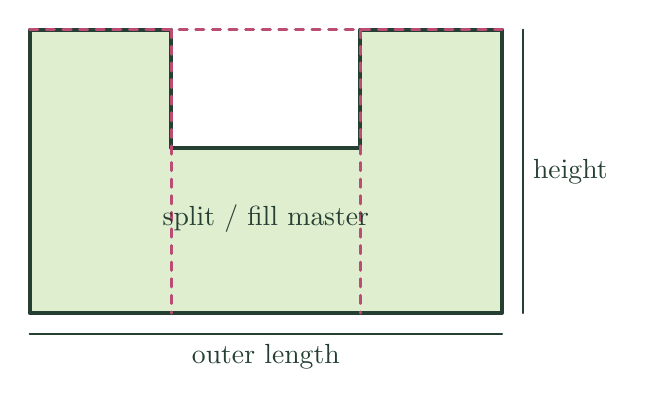
\begin{tikzpicture}[x=0.6cm,y=0.6cm,line cap=round,line join=round]
  \filldraw[fill=surface,draw=outline,line width=1.4pt]
    (0,0)--(0,6)--(3,6)--(3,3.5)--(7,3.5)--(7,6)--(10,6)--(10,0)--cycle;
  \draw[guide,dashed,line width=1pt] (0,6)--(10,6) (3,6)--(3,0) (7,6)--(7,0);
  \draw[outline,line width=.8pt] (0,-.45)--(10,-.45);
  \node[below,text=outline] at (5,-.45) {outer length};
  \draw[outline,line width=.8pt] (10.45,0)--(10.45,6);
  \node[right,text=outline] at (10.45,3) {height};
  \node[text=outline] at (5,2) {split / fill master};
\end{tikzpicture}
\end{document}
